\documentclass[12pt]{unlsilabsop}
\title{Functionality Test of DTB and Voltage Power Supply}
\date{September 10, 2015}
\author{Joaquin Siado, Frank Meier Aeschbacher}
\approved{Frank Meier Aeschbacher}
\sopid{207}
\sopversion{v1}
\sopabstract{Describes the procedures for doing a functionality test a DTB and a voltage power supply (VPS). This consists of measuring analogue and digital current for a DTB and current for a power supply. Any deviations from normal appearance will be documented.}
\newcommand{\at}{\makeatletter @\makeatother}
\begin{document}

\maketitle

%------------------------------------------------------------------
\section{Scope}
This is a regular test in the manufacturing process of pixel modules at UNL. This test should be done before a module testing session is started

%------------------------------------------------------------------
\section{Purpose}
The functionality test of a DTB and VPS is a critical step in manufacturing modules. This test is a critical control point to make sure the material we send out meets expectations and to ensure the quality. 

%------------------------------------------------------------------
%>\section{Definitions}

%------------------------------------------------------------------
%\section{Responsibilities}

%------------------------------------------------------------------
\section{Equipment}

\begin{itemize}
\item \textbf{DTB} Power up and connected to the computer
\item \textbf{DTB tester} A board consisting of a set of resistors specially design to measure currents of the DTB
\item \textbf{Computer} A Linux or Mac~OS~X based computer with pXar installed.
\item \textbf{HV power supply} Keithly model 2410, connected to the same computer through a USB to RS232 adapter. Do not turn it on until it is necessary.
\item \textbf{Binder clips} 15\,mm wide, inside insulated with Kapton tape.
\end{itemize}

%------------------------------------------------------------------
\section{Procedure}
\begin{figure}[hhhh]
\begin{center}
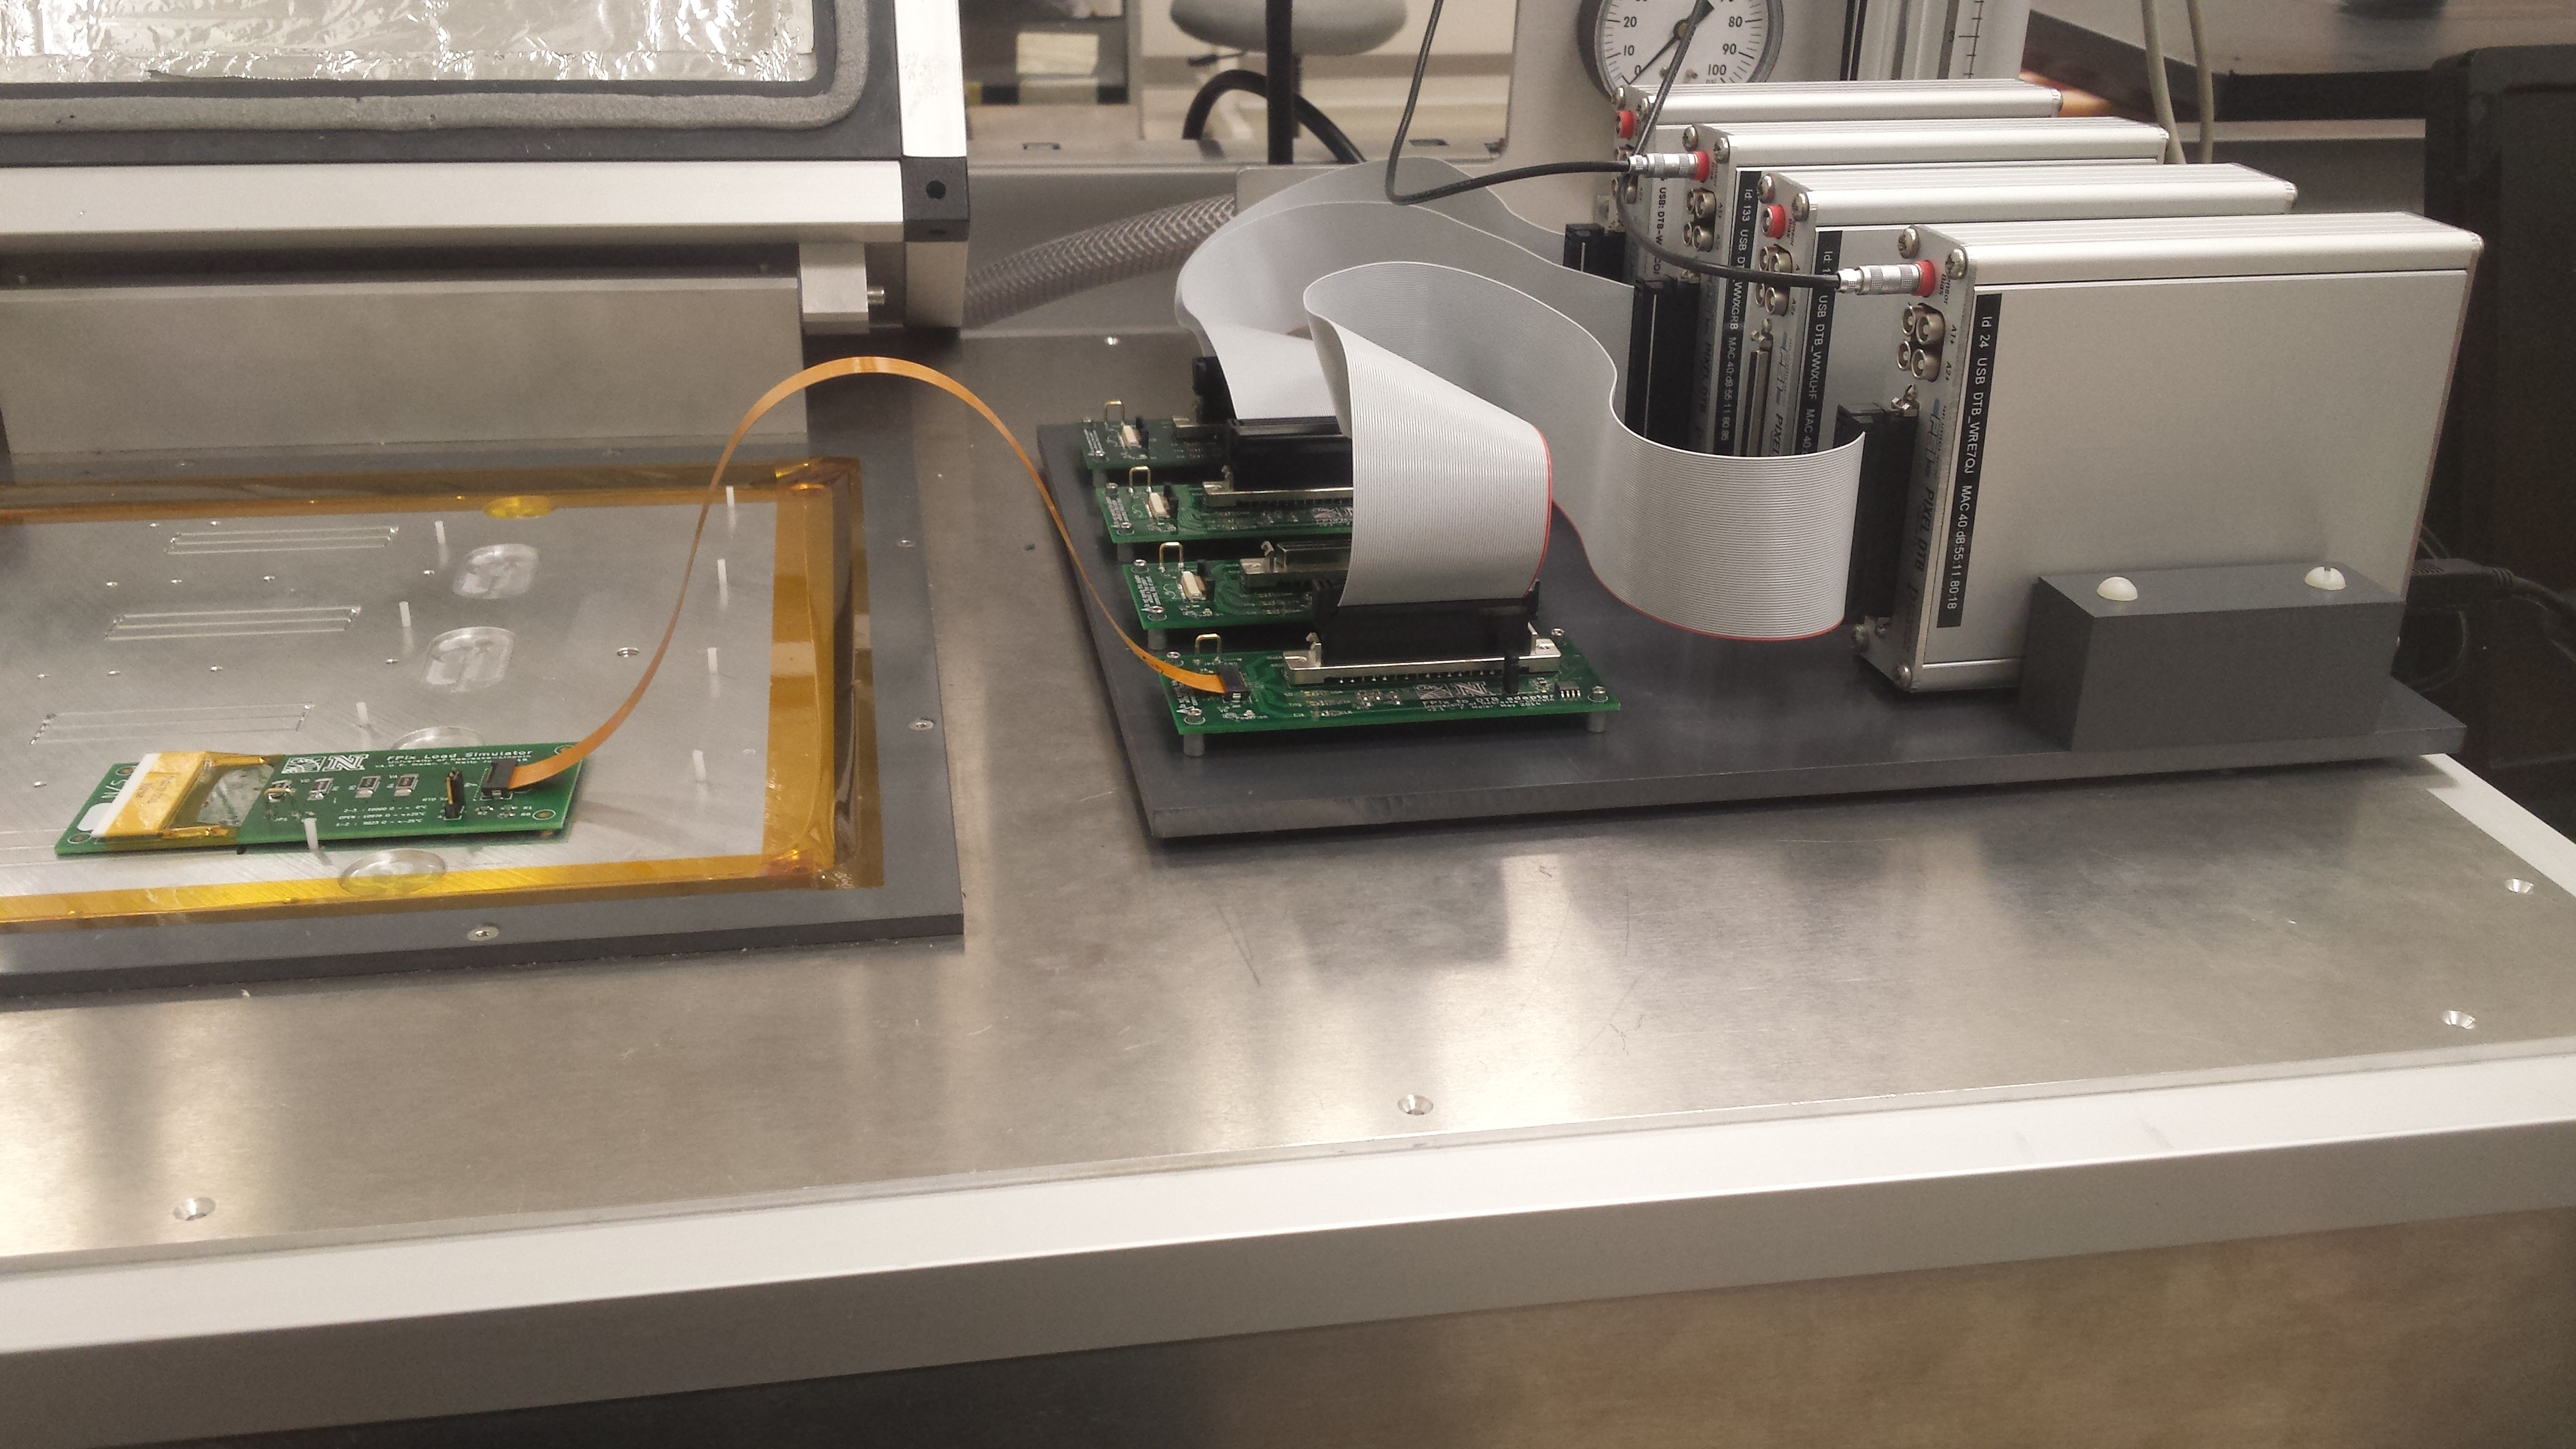
\includegraphics[scale=0.05]{img/DTB_2}
\vspace{0.5cm}
\caption{DTB tester connected to a DTB for a functionality test.}
\label{dtb}
\end{center}
\vspace{1cm}
\end{figure}

\begin{enumerate}
    \item Handle modules only with proper protection: ESD wristband, gloves, face mask (if needed).
    \item A protective Kapton-insulated binder clip has to be attached to the dangling end of the flex cable whenever modules are stored or handled when no ESD protection can be worn (e.g.~when transferring modules on closed carriers between cleanroom and test stand).
    \item Connect the DTB tester to a DTB, as shown in Figure ~(\ref{dtb}) .
    \item star pxar software and read analogue and digital current from the pxar gui. If the current are within range, 1.1 for both quantities, move to the next step. Otherwise close pxar gui immediately.
    \item Turn on the VPS and read the current, it should be around 6 $\mu A$, turn it off as quickly as possible.
    \item Quit the pxar gui by clicking the exit button.
    \item Repeat this process for all needed DTB and VPS.
	\item Disconnect the DTB tester, place the binder clip on, and store it in a safe place.  	
    \item Document any findings.
\end{enumerate}

%------------------------------------------------------------------
\section{Documentation}
Date of the test, DTB's id, Analogue current, digital current, current of the VPS. Add any other information you considered relevant.

\end{document}

